\section{Listener\-Base Class Reference}
\label{classListenerBase}\index{ListenerBase@{ListenerBase}}
Inheritance diagram for Listener\-Base::\begin{figure}[H]
\begin{center}
\leavevmode
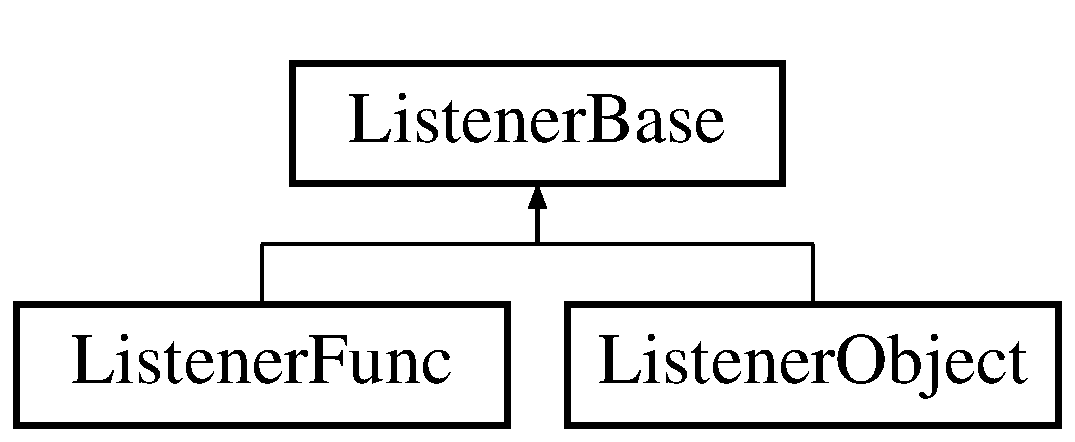
\includegraphics[height=2cm]{classListenerBase}
\end{center}
\end{figure}
\subsection*{Public Member Functions}
\begin{CompactItemize}
\item 
{\bf invoke} ()
\end{CompactItemize}


\subsection{Member Function Documentation}
\index{ListenerBase@{Listener\-Base}!invoke@{invoke}}
\index{invoke@{invoke}!ListenerBase@{Listener\-Base}}
\subsubsection{\setlength{\rightskip}{0pt plus 5cm}Listener\-Base::invoke ()}\label{classListenerBase_ListenerBasea0}




Reimplemented in {\bf Listener\-Object} {\rm (p.\,\pageref{classListenerObject_ListenerObjecta0})}, and {\bf Listener\-Func} {\rm (p.\,\pageref{classListenerFunc_ListenerFunca1})}.

The documentation for this class was generated from the following file:\begin{CompactItemize}
\item 
{\bf Listener.py}\end{CompactItemize}
